\documentclass{article}
\usepackage{graphicx}
\usepackage{hyperref}
\usepackage[parfill]{parskip}

\setlength{\oddsidemargin}{0in}
\setlength{\evensidemargin}{0in}
\setlength{\textwidth}{6.5in}
\setlength{\topmargin}{-0.75in}
\setlength{\textheight}{9.25in}
\hypersetup{colorlinks = true, urlcolor = blue}

\begin{document}

\title{Kimbee: A Speech Therapy Application For Children}
\author{Ryan Drapeau \and Nick Huynh \and Aaron Nech}
\date{\{drapeau, necha, huynick\}@cs.washington.edu}

\maketitle

\section{Abstract}

Many kids have difficulty pronouncing certain sounds and their parents are forced to pay for speech therapy for their children. We hope to create a web application that doubles as a game in order to help children who are undergoing speech therapy recognize and pronounce certain sounds. The game should keep children wanting to play more, making their speech therapy seem like less of a chore and help them learn by having the children try say the word then correct or reward them depending on their pronunciation. We will speak with a professional speech therapist in order to help shape our game and the feedback it gives back to children in order to give more constructive feedback than simply repeating the correct pronunciation back to them.

\section{Scenarios and Goals}

A child has difficulty pronouncing and differentiating the ``l'' and ``r'' sounds. He or she goes to speech therapy but in order to reinforce his or her learning, he or she can use Kimbee. Before starting, his or her mother or father can pick the setting designed to help correct ``l'' and ``r'' sounds then let him or her play Kimbee. He or she will hear a word, say it back and depending on his pronunciation, advance in the game or have the word repeated back at him or her until he learns.

\section{Design Strategy}

\centerline{\textbf{Main Components}}

\begin{tabular}{cc}
    \centering
    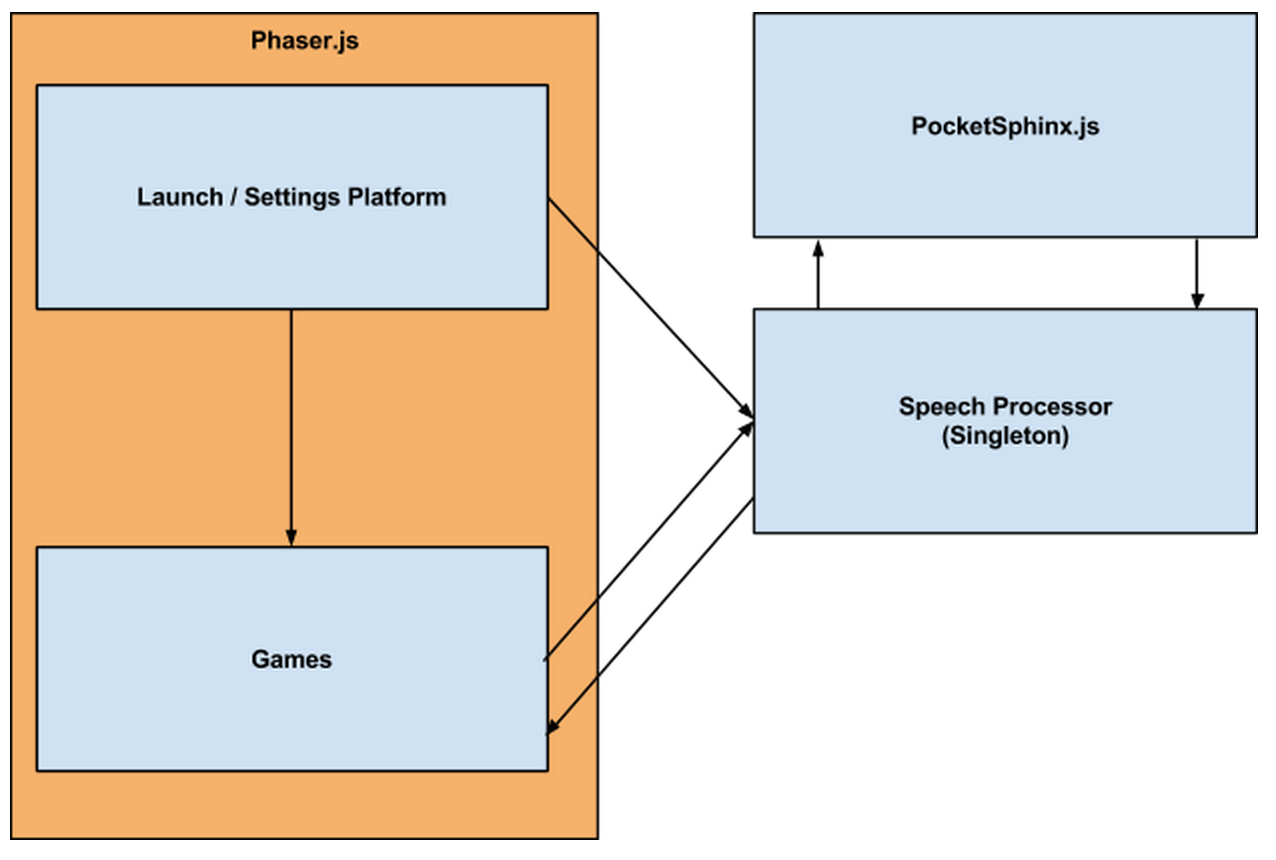
\includegraphics[width=0.46\textwidth]{outline.png} & 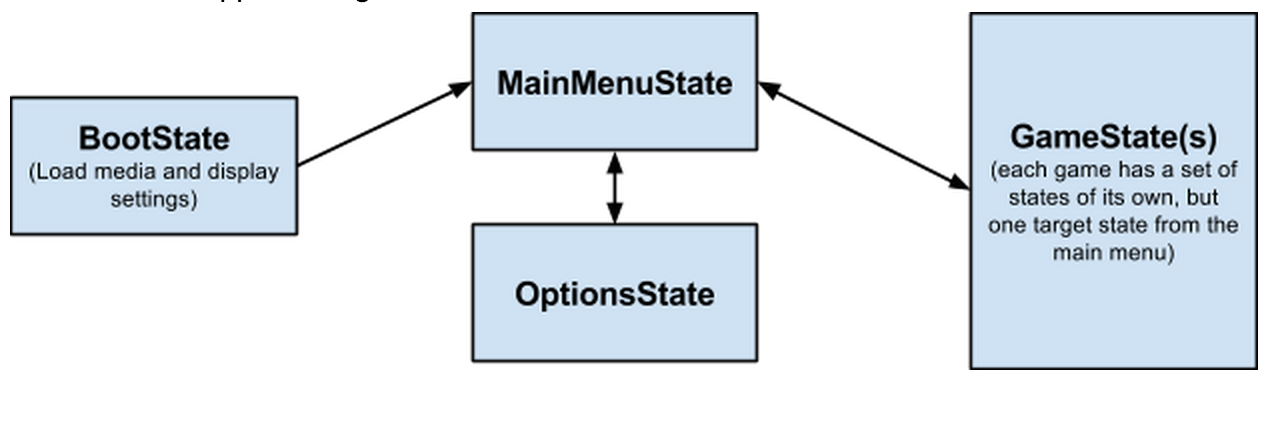
\includegraphics[width=0.5\textwidth]{states.png}\\
    Figure 1 & Figure 2
\end{tabular}

\newpage

\href{http://syl22-00.github.io/pocketsphinx.js/}{\textbf{PocketSphinx.js}}\\
An open source port of CMU pocket-sphinx to javascript that will serve as our sound processing backend.

\textbf{Speech Processor}\\
A set of software built on top of (and interfaces with) the PocketSphinx.js library. This will be the set of software that our game(s) communicates with while playing. This will also track performance on certain words. This set of software will also serve words to the game upon request (i.e, getNextWord()).

\href{http://phaser.io/}{\textbf{Phaser.js}}\\
The game framework we will utilize to manage game state, media assets, and user interactivity. This framework is a good choice because it allows multiple platform targets for our final product.

\textbf{Game(s)}\\
A series of bee-themed mini games (one or more depending on how far we get), that utilize the Word Processor described above as a central part of gameplay for practicing speech.

\textbf{Launch / Settings Platform}\\
The entry point of our application where the games are launched from. This will also contain options for selecting certain key sounds (``L'' and ``R'' at first), selecting these options will interact with the \textit{Word Processor} ultimately configuring it for the \textit{Game(s)}. Implementation wise, this is analogous to our main menu.

The interactions between all of these components are shown in Figure 1.

\section{Implementation Details}

\textbf{States}\\
The flow of the application will be modeled with Phaser states. See Figure 2.

\textbf{Speech Processor}\\
The main internal speech processor API will be constructed as a singleton object. This will be a interface that is a composite of many objects that run and manage the speech therapy part of the game. The game states above will interact with this singleton through its interface. Exact architecture of the speech processor is yet to be determined, but will interact with the PocketSphinx.js library.

\section{Unkowns and Risks}

Recognizing the difference between a correct pronunciation and an incorrect one. Designing a game geared towards kids that they will enjoy. Giving feedback when a child gives an incorrect answer that is constructive and assists their learning further than just repeating the word back to them.

\section{Implementation Plan and Schedule}

\begin{enumerate}
    \item Application scaffolding (game structure, menu, options) (Week 4)
    \begin{enumerate}
        \item Create phaser.js application
        \item Create game states listed above in this project specification
        \item Setup main menu with game launching capabilities
        \item Create SpeechProcessor singleton and associated speech module classes
    \end{enumerate}
    \item Simple game screen to connect to speech API for testing (Week 4)
    \begin{enumerate}
        \item Create simple game, and hook up to launcher created in (1)
        \item Connect API calls to fetch next available therapy word
        \item Connect API calls to start and stop microphone data gathering through a phaser based object that materializes as a microphone start/stop button
        \item Connect API calls to process data
        \item Connect API calls to determine success or failure on pronunciation
        \item Place (a)-(d) in an iterative game loop with some termination amount until game completion
        \item After game completion, move user to completed screen, and allow returning to launch menu defined in (1)
    \end{enumerate}
    \item Contact therapists and refine project goals / industry need (Week 6)
    \begin{enumerate}
        \item Email therapist
        \item Set up meetings to learn about current processes and how to best target our project
    \end{enumerate}
    \item Web Audio API, Microphone capture, Data pipeline in javascript (Week 6)
    \begin{enumerate}
        \item Create module/class interfaced by (2) through the API singleton created in (1) to store and manipulate therapy settings
        \item Create module/class interfaced by (2) through the API singleton created in (1) to get next word based on settings defined in (a)
        \item Create module/class interfaced by (2) through the API singleton created in (1) to gather microphone audio feedback and return it
    \end{enumerate}
    \item Speech, phoneme recognition in javascript with pocketsphinx.js (Week 6)
    \begin{enumerate}
        \item Create module/class interfaced by (2) through the API singleton created in (1) to take microphone feedback and compute phoneme translation confidences with pocketsphinx.js and the phoneme translator model
        \item Create module interfaced by (2) through the API singleton created in (1) to process phoneme confidences produced by (d) and return a success or failure based on settings stored in (4a) and defined by the user through the option menu specified in (1)
    \end{enumerate}
    \item Progress tracking metrics related to confidence data on child performance (Week 8)
    \begin{enumerate}
        \item Create ProgressTracker object that will be composited in the SpeechProcessor singleton
        \item Hook up this tracker object to intercept API calls on SpeechProcessor and record progress on metrics determined in (3)
        \item Create screen attached to option menu to display progress stored in (a)
        \item Create web server endpoints to store child data and accessible by therapist (this a further goal)
        \item Further machine learning, predictions, etc on the data as therapist suggests
    \end{enumerate}
    \item Iterate specific progress tracking implementations with therapist feedback (Week 8)
    \begin{enumerate}
        \item Stay in contact with therapist and show them how our work progresses
    \end{enumerate}
    \item More games that utilize javascript speech API defined in the above sections (Week 10)
    \begin{enumerate}
        \item Create a maze based game (idea 1)
    \end{enumerate}
    \item Polish everything, animations, graphics, sound etc. (Week 10)
    \begin{enumerate}
        \item Check for bugs, issues, screen transition problems
        \item Test speech api extensively until it is smooth
        \item Gather feedback from therapist and maybe children
        \item Spend a lot of effort polishing art work, game tweens, animations, and sound
    \end{enumerate}
    \item Package up to apps and deliver to app store (Week 10)
    \begin{enumerate}
        \item Use phaser.js and phone pipelines that exist
        \item Create app icons, splash screens, and other necessary app store content
    \end{enumerate}
    \item Write up / Poster (Week 11)
\end{enumerate}

\section{Evaluation}

We will try to meet with a speech therapist to see if they will implement Kimbee as part of their therapy course or if they can recommend it to their patients. We will be successful if we provide a game that the kids can learn from and a game that they will enjoy playing. We can measure the first by tracking a child's feedback and seeing if their responses become clearer as time moves on and the second by measuring how much a child is using the app per week. By charting multiple childrens' feedback, we can display their learning on our final report and evaluate whether or not a game setting was appropriate or not for helping children learn.

\section{Related Work}

\href{https://itunes.apple.com/us/app/articulation-station-pro/id491998279}{Articulation Station Pro}\\
``Learn how to pronounce and practice the consonantal sounds in the English language...''\\\\
Although this application helps young children learn how to pronounce and dictate words, it was not made with children with speech disorders in mind. Our application will have a setting which will allow the user or speech therapist the ability to change the part of speech that is being addressed in the game. We might also explore the possibility of developing a model of each user's speech to gain insight into every person that uses Kimbee. This will allow us to track the user’s performance over time as he or she continues to use the application.\\[25 pt]
\href{http://dihana.cps.unizar.es/~alborada/docu/2006cvaquero.pdf}{Vocaliza}\\
``The objective of this application is to help the daily work of the speech therapists that train the linguistic skills of Spanish speakers with different language pathologies.''\\\\
Unfortunately, as mentioned at the end of this paper, this application failed to create a game that was intuitive for children to play. Although the authors designed an impressive system for modeling user speech, the “game” wasn’t anything of the sort. Vocaliza allowed users to select a word and then practice speaking it over and over. This did not include any game like mechanics. Kimbee will be a progressive move based game where the user can earn more moves by performing better in speech.\\[25 pt]
\href{http://www.speech.kth.se/prod/publications/files/841.pdf}{OLP (Ortho-Logo-Paedia)}\\
``This paper presents an overview of a newly started EU-funded research project and outlines the design of the speech therapy structure to be used within the project.''\\\\
This paper addresses the fact that having a visual feedback system is important for children to be able to learn and improve their speech. However, it fails to provide a solution. Kimbee will be a tool to help children with speech impediments wrapped around a game that provides the user with feedback. For example, the user could attain a move to use every time they score high on a word or sentence. This would keep the child or user entertained and engaged while they used the application and it provides motivation to improve and do better.

\end{document}
